\chapter{Krav}

Ud fra projektformuleringen er der formuleret en række krav til projektet. Disse indebærer to use cases og et antal ikke-funktionelle krav. 


Indsæt figur her. 

%
%\begin{figure}[H]
%	\centering
%	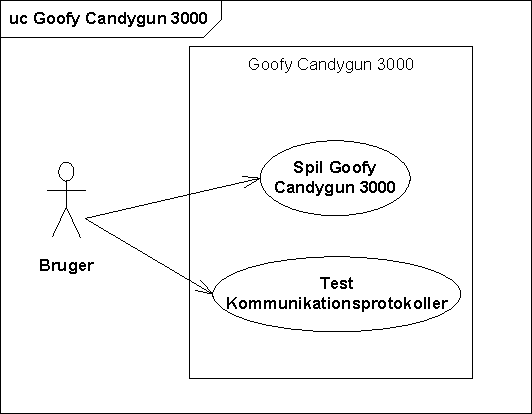
\includegraphics[width=0.80\textwidth]{images/usecaseDiagram.png}
%	\caption{Use case diagram}
%	\label{fig:sketch}
%\end{figure}


\section{Aktørbeskrivelse}
På figur 1 ses aktør-kontekst-diagrammet for systemet. På dette ses det, at der i systemet er en enkelt aktør og to use cases. Den ene aktør er brugeren som samtidig er den primære aktør. Brugeren kan sætte de to use cases i gang, hvilket indebærer, at kunne spille Goofy Candygun 3000 og sætte en test af systemet i gang. 

\section{Use case beskrivelse}
\subsection{Use case 1}
Dette er den rigtige use case. Det er denne, der køres, når der skal spilles et spil på Goofy Candygun 3000, og den initieres af brugeren. Det første der sker i use case er, at brugeren skal vælge, hvilken type spil han/hun gerne vil spille. Det betyder, at det skal bestemmes, om det skal være et enpersonsspil, topersonersspil eller om det skal være party mode. Herefter skal der vælges, hvor mange skud et spil skal vare og disse skal puttes i magasinet. Når dette er gjort kan spillet gå i gang. Brugeren indstiller kanonen med Wii-nunchuck og affyrer den. Herefter lader systemet et nyt skud og samme procedure gentages. Til slut vises information om spillet på brugergrænsefladen, brugeren afslutter spillet ved at trykke på knappen på brugergrænsefladen og denne vender tilbage til starttilstanden. 

\subsection{Use case 2}
Use case 2 skal kun bruges til at teste systemet og dets kommunikationsprotokoller. Den skal bruges til at finde ud af om systemet virker og hvis det ikke gør, hvad det så er, der er gået galt og hvor det er gået galt. Use casen initieres af brugeren, hvor der herefter bliver sendt informationer ud til de forskellige dele af systemet, som så gerne skal sende svar tilbage igen. Hvis det sker for alle dele, vil brugergrænsefladen til sidst meddele, at use casen er gennemført. 


\section{Ikke-funktionelle krav}
De ikke-funktionelle krav siger noget om, hvordan systemet skal bygges, og hvilke specifikationer det skal have. I dette tilfælde er der udarbejdet syv krav, hvor der er et der siger noget om, hvordan kanonen skal kunne drejes. Nogle siger noget om kanonens størrelse, hvor der også er specificeret, hvor stort projektilet den skal affyre må være og et siger, hvor langt den skal kunne skyde. Der er et, der siger, hvor lang tid det må tage at skyde et projektil afsted og hvor hurtig den skal være til at lade kanonen igen. Endelig er der et, der specificerer, hvordan den grafiske brugergrænseflade skal se ud. Deciderede værdier for de enkelte krav kan læses i bilag. 







